\section{Deskriptor}
En Deskriptor modtager en række koordinater fra detektoren, som er vurderet til at være interessante.
Disse koordinater repræsentere et subset af billedet, hvor der ifølge detektoren opstår interessepunkter, dette kan f.eks. være hjørner fra en hjørnedetektor. 
 Det er nu deskriptorens opgave at knytte en beskrivelse til hvert punkt. Denne beskrivelse kommer ofte i form af en x-dimensional vektor\footnote{For en given metode vil længden af disse vektorer altid være ens}, hvor indgangende i vektoren bærer noget karakteristisk information om interessepunktet, det kunne f.eks. være gradient retninger af et $n \times n$ område omkring interessepunktet.
Vektorene kan dernæst bruges til at determinere, hvor ens to punkter er og derved bestemme om punkterne korrespondere. I sektion \ref{sec:detect} defineres et interessepunkt bl.a. som værende distinkt ift. de omkringliggende pixels og lokaliseret i et område, hvor der sker store intensitetsskift. Dette hjælper deskriptoren i at kunne bruge den omliggende region til at beskrive punktet. En simpel metode at beskrive et interessepunkt, er at tage området omkring punktet, gemme disse værdier i en vektor og sammenligne afstanden fra denne vektor med alle andre beskrivelser af interessepunkter, i det andet billede. Dette kan være fordelagtigt, hvis de to billeder ikke er udsat for nogen ændring, andet end forkydelse af kameraet. Men da billederne næsten i alle sammenhæng med fotografering,undtagen i meget kontrollerede forhold, udsættets for mange ændringer, når kameraet skifter position, vil denne løsning ikke virke. Generelt ønskes der at en deskriptor besidder følgende egenskaber:
\begin{itemize}
\item{ \textit{Uafhængig af interessepunktets placering}
Bliver interessepunktet udvundet på forskellige position  (f.eks. pga. bevægelse af kameraet ift. scenen) skal deskriptoren være ens og derved kunne identificer disse som korresponderende punkter
 }
\item{\textit{Robust} Deskrpitoren skal kunne identificere to korresponderende punkter som værende ens på trods af transformationer i billedet, bl.a. ændringer i lys, perspektiv}
\item{\textit{Invariant} Deskriptoren skal være invariant overfor ændringer i skala, rotation o.s.v. Invarians kan opnås ved at identificere ændringer, kompensere for disse og derefter beskrive området.
Hvordan en deskriptor kan opnå rotationsinvarians er bekrevet herunder.}
\end{itemize}
Er der sket en rotation af det ene billede ift. det andet, kan deskriptoren kompensere for dette. Dette kan udføres ved at finde den dominerende gradient i pixelområdet omkring interessepunktet og derved punktets orientering. Regionen kan dernæst roteres ift. punktets orientering så alle regioner har samme rotation \cite{bjerg}. Dette er illustreret i figur \ref{fig:bjerg}, hvor regionen omkring et interessepunkt er roteret relativt til interessepunktets orientering.
\begin{figure}[H]
    \centering
    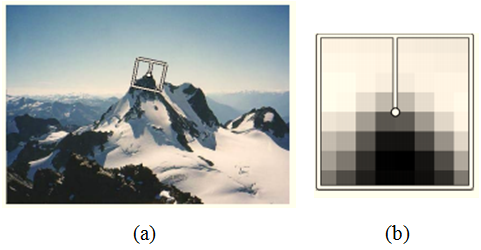
\includegraphics[width=0.45\textwidth]{fig/21.png}
    \vspace{-0.5em} 
    \begin{center}
    \caption{\textcolor{gray}{\footnotesize \textit{
   (a) Et interessepunkt lokaliseret på en bjergtop,  repræsenteret af en firkant, med centrum i interessepunktet og en lodret streg der angiver punktets rotation. (b) Interessepunktet forstørret i et 8x8 pixel område, hvor rotationen af punktet er trukket fra og derfor normaliseret.}}}
    \label{fig:bjerg}
     \end{center}
  \end{figure}
       \vspace{-2.5em}
\noindent
Selv efter kompensering for rotation, skala o.s.v. vil korresponderende regioner stadig variere ift. til hinanden. Udfordringen består derved i at deskriptoren skal være invariant overfor ændringer så korresponderende punkter kan matches korrekt(sand positiv), men også informationsbærende/unikke nok, så der ikke opstår forkerte korrespondancer (falske positive). Der er mange forskellige måder at beskrive interessepunkter og dertil mange forskellige deskriptorer, der hver især beskriver området forskelligt. I udvælgelsen af en deskriptor skal der tages højde for følgende:
\begin{itemize}
\item{ \textit{Information} Hvad deskriptoren skal bruge til at karakterisere området med. Det kan f.eks. være farve, tekstur, gradient orientering el.a.}
\item{ \textit{Kompleksitet}Hvor distinkt skal deksriptoren være, altså hvor meget information deskriptoren skal indeholde. Dette er ofte defineret ift. hvor stor en dimension vektoren har. Der er her et "trade-of" imellem, hvor beskrivende deskriptoren skal være og hvor lang tid det må tage at udregne deskriptoren da udredningstiden stiger med udvidet kompleksitet.}
\end{itemize}
Ovenstående skal besluttes ift. applikationsdomænet altså, hvad billederne forestiller, og hvor hurtigt den skal være at udregne. \\
<Måske lidt om gradient baseret deskriptorer>